% Created 2019-06-21 ven. 11:46
\documentclass{article}
\usepackage[utf8]{inputenc}
\usepackage[T1]{fontenc}
\usepackage{fixltx2e}
\usepackage{graphicx}
\usepackage{longtable}
\usepackage{float}
\usepackage{wrapfig}
\usepackage{rotating}
\usepackage[normalem]{ulem}
\usepackage{amsmath}
\usepackage{textcomp}
\usepackage{marvosym}
\usepackage{wasysym}
\usepackage{amssymb}
\usepackage{hyperref}
\tolerance=1000
\usepackage[frenchb]{babel}
\date{\today}
\title{TP2 : Tkinter}
\hypersetup{
  pdfkeywords={},
  pdfsubject={},
  pdfcreator={Emacs 25.2.2 (Org mode 8.2.10)}}
\begin{document}

\maketitle


\section{Présentation Tkinter}
\label{sec-1}
Tkinter est un outil de représentation graphique facile à prendre en main et disponible dans la librairie standard Python.

\noindent
L'objet \verb~Tk~ est celui qui crée la fenêtre principale de l'application.

\noindent
Dans la plupart des objets tkinter on peut ajouter de nombreux \emph{Widgets}, ce sont des objets comme des boutons (\verb~Button~), des étiquettes (\verb~Label~) ou des champs de saisie (\verb~Entry~).
Une fois ces \emph{Widgets} créés, il faut le placer dans la fenêtre avec l'opérateur de placement \verb~.pack()~

\noindent
Pour tout renseignement supplémentaire, vous pouvez utiliser \verb~help()~ dans la console ou aller sur le site \url{http://tkinter.fdex.eu} .

\section{Ma première fenêtre}
\label{sec-2}
Pour créer votre première fenêtre, il vous suffit d'importer tkinter avec la commande:
\begin{verbatim}
import tkinter as tk
\end{verbatim}

Il vous suffit alors de créer une nouvelle application en créant un objet de type \verb~tk.Tk~ et de le lancer avec la méthode \verb~.mainloop()~.

\noindent
/!$\backslash$ Prenez bien note de lancer la \verb~.mainloop~ en dernier, car il est bloquant.


\noindent
Vous pouvez ensuite commencer à modifier les paramètres de la fenêtre
\begin{itemize}
\item \verb~.title(str)~ : Change le titre de la fenêtre
\item \verb~.geometry(str)~ : Change la taille de la fenêtre et son emplacement sur l'écran
\end{itemize}

\noindent
Pour ajouter un bouton, il suffit de créer un objet \verb~Button~ avec comme premier paramêtre l'objet \verb~Tk~ pour qu'il lui soit rattaché.
On peut modifier le texte du bouton avec l'option \emph{text} à l'initialisation (exemple: \verb~Button(fenetre,text="Texte")~).

\noindent
On donne également la fonction à éxécuter avec l'option \emph{command} dans l'initialisation. Il faut passer la fonction sans les parenthèses, ce qui limite les fonctions possibles aux fonctions sans paramètres. La fonction à utiliser pour fermer une fenêtre est \verb~fenetre.destroy()~.


\noindent
Vous pouvez maintenant créer une fenêtre possédant un bouton pour pouvoir la fermer. Elle devrait ressemble à celle-ci:

\begin{center}
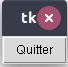
\includegraphics[width=.3\linewidth]{./img/premiereFenetre.png}
\end{center}

\section{Les canvas}
\label{sec-3}
Le \verb~Canvas~ est un \emph{Widget} servant principalement à contenir des dessins.
Pour dessiner dans le canvas vous pouvez utiliser les commandes suivantes:
\begin{itemize}
\item \verb~create_arc()~: permet de dessiner un arc de cercle
\item \verb~create_line()~: permet de dessiner une ligne
\item \verb~create_oval()~: permet de dessiner un cercle ou un ovale
\item \verb~create_rectangle()~: permet de dessiner un rectangle
\item \verb~create_polygon()~: permet de dessiner un polygone
\end{itemize}

\noindent
La plupart de ces fonctions demandent la zone dans laquelle la forme doit être dessinée.
Les informations demandées sont le point en haut a gauche (\verb~x0~, \verb~y0~), le point en bas à droite (\verb~x1~, \verb~y1~), et des options additionnelles pouvant être spécifiques à chaque forme.

\noindent
$\backslash$/!$\backslash$ Notez que le point en haut à gauche de la fenêtre est de coordonnées (0,0) et que l'axe des \emph{x} est sur la hauteur

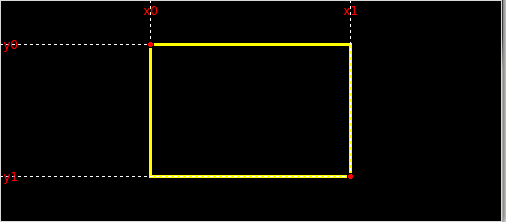
\includegraphics[width=.9\linewidth]{./img/coord_canvas.png}

\noindent
Chaque élément dessiné dans le Canvas pourra ensuite être déplacé ou supprimé du Canvas grâce aux méthodes \verb~move~ et \verb~delete~.
Pour pouvoir utiliser ces méthodes, il vous faudra avoir récupéré l'identifiant de ces éléments qui est donné lorsqu'ils sont créés.

\section{Le labyrinthe}
\label{sec-4}

À partir du tableau donné dans le fichier \emph{labyrinthe.py}, créer une fenêtre tkinter où les -1 sont représentent des carrés noirs et les 0 des carrés blancs.
Notez bien que le tableau est haut de 31 ligne et large de 28 colonnes.

\noindent
Pour diminuer le travail à réaliser, vous pouvez entrer l'option \emph{bg} à l'initialisation du \verb~Canvas~ pour spécifier la couleur de son fond (couleur à donner en anglais, entre guillemets).

\noindent
Votre travail devrait ressembler à ceci:

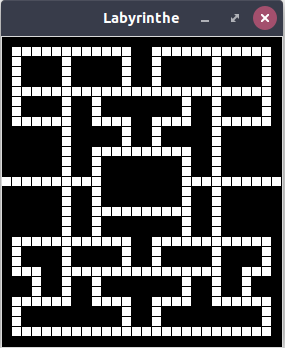
\includegraphics[width=.9\linewidth]{./img/labyrinthe.png}
% Emacs 25.2.2 (Org mode 8.2.10)
\end{document}